%%%%%%%%%%%%%%%%%%%%%%%%%%%%%%%%%%%%%%%%%%%%%%%%%%%%%%%%%%%%%%%%%%%%%%
% LaTeX Template: Project Titlepage
%
% Source: http://www.howtotex.com
% Date: April 2011
%
% This is a title page template which be used for articles & reports.
%
% Feel free to distribute this example, but please keep the referral
% to howtotex.com
%
%%%%%%%%%%%%%%%%%%%%%%%%%%%%%%%%%%%%%%%%%%%%%%%%%%%%%%%%%%%%%%%%%%%%%%
%
% --------------------------------------------------------------------
% Preamble
% --------------------------------------------------------------------

\documentclass[paper=a4, fontsize=11pt,twoside]{scrartcl}       % KOMA

\usepackage[a4paper,pdftex]{geometry}   % A4paper margins
\setlength{\oddsidemargin}{5mm}                 % Remove 'twosided' indentation
\setlength{\evensidemargin}{5mm}

\usepackage[english]{babel}
\usepackage[font=footnotesize, labelfont=it]{caption}
\usepackage[protrusion=true,expansion=true]{microtype}
\usepackage{mathtools}
%\usepackage{tikz-network}
\usepackage{graphicx}
\usepackage{wrapfig}
\usepackage{subfig}
\usepackage{amsfonts}
\usepackage[backref=true, sorting=none]{biblatex}
\usepackage{csquotes}
\addbibresource{bibliography.bib}
\usepackage{hyperref}
\hypersetup{
        colorlinks=true,
        linkcolor=blue,
        filecolor=magenta,
        urlcolor=blue,
        citecolor=blue
        }
\urlstyle{same}

% --------------------------------------------------------------------
% Definitions (do not change this)
% --------------------------------------------------------------------

%Command for beginning supplementary tables & figures
\newcommand{\beginsupplement}{
        \setcounter{table}{0}
        \renewcommand{\thetable}{S\arabic{table}}%
        \setcounter{figure}{0}
        \renewcommand{\thefigure}{S\arabic{figure}}%
     }

\newcommand{\HRule}[1]{\rule{\linewidth}{#1}}   % Horizontal rule

\makeatletter                                                   % Title
\def\printtitle{%
    {\centering \@title\par}}
\makeatother

\makeatletter                                                   % Author
\def\printauthor{%
    {\centering \large \@author}}
\makeatother

% --------------------------------------------------------------------
% Metadata (Change this)
% --------------------------------------------------------------------

\title{
%                        \HRule{0.5pt} \\                                                % Upper rule
                        \LARGE \textbf{\uppercase{A Computationally Tractable Model for the Evolution of a Genome's Size and its Growing Fitness Landscape}}      % Title
%                        \HRule{2pt} \\ [0.5cm]          % Lower rule + 0.5cm spacing
%                        \normalsize \today                      % Todays date
                }

\author{
                \textbf{Master's Thesis}\\
                Faculty of Science, University of Bern\\
                \vspace{1cm}
                Handed in by \\
                \textbf{Jacob Hugh Riina} \\
		\vspace{2cm}
		\textbf{2025}
                \vfill
                Supervisor\\
                Prof. Dr. C. Bank\\
                Dr. S. Peischl\\
}

\begin{document}

% ------------------------------------------------------------------------------
% Maketitle
% ------------------------------------------------------------------------------

\thispagestyle{empty}           % Remove page numbering on this page

\printtitle                                     % Print the title data as defined above
        \vfill
\printauthor                            % Print the author data as defined above
\newpage

% ------------------------------------------------------------------------------
% Begin document
% ------------------------------------------------------------------------------

\setcounter{page}{1}            % Set page numbering to begin on this page

\section*{Introduction}

\subsection*{Genome Evolution}

Since life's origins approximately 3.5 billion years ago it has generally increased in complexity, and understanding the processes that generate this complexity is one of the main goals of evolutionary biology \cite{duclosInvestigatingEvolutionDevelopment2019}\cite{mcshea2010biology}. One such mechanism of generating complexity is through genome evolution \cite{lynchOriginsGenomeComplexity2003}: by changing the size of their genomes, the earliest living cells - those with a cell membrane, which encode and pass on information through their DNA - were able to create \textit{evolutionary innovations}\cite{wagnerMolecularOriginsEvolutionary2011}: new metabolism, physiology or regulation, which augmented their ability to thrive in a variety of environments \cite{barveLatentCapacityEvolutionary2013}\cite{uebbingEvolutionaryInnovationsConserved2024}. At the increased cost of replicating and proofreading more DNA, organisms have since been able to evolve new genes allowing them to metabolize different carbon, nitrogen, or complex nutrient sources, various types of receptors and secretion systems to interact, competitively or mutualistically, with others, and the internal regulatory networks required for them to decide which behaviors are optimal under which circumstances, or even to coordinate multicellularity. Several billion years later, we see the consequences of this incessant evolutionary process: the stunning diversity amongst organisms in the tree of life, each a product of the series of environments they have adapted to. We can say, then, that the content of an organism's genome is not solely the result of how it has evolved to fit its current environment, but also the entire history of environments that its ancestors have evolved in; as always, "Nothing in biology makes sense except in the light of evolution" \cite{dobzhanskyBIOLOGYMOLECULARORGANISMIC1964}.

Understanding this facet of evolution is difficult. Unlike with the point mutations that are typically observed in every generation, genome evolution occurs up to several orders of magnitude less frequently \cite{sousaRatesTranspositionEscherichia2013}\cite{lipinskiHighSpontaneousRate2011}, and is more heterogenous in its manifestation. We define here \textit{genome evolution} as a mutational process resulting in either the expansion or reduction in the size of the functional genome, arising from one of several causes: amongst genome-increasing mechanisms, there exist duplications from repeat region replication errors \cite{reamsMechanismsGeneDuplication2015}, transposon activity, or whole genome duplications (WGD), as well as genes arising from noncoding sequence through de novo gene birth \cite{sacconeOriginEvolutionGenes2025}, while genome-reducing mechanisms include pseudogenization and deletions via various types of replication errors \cite{burssedMechanismsStructuralChromosomal2022}. Evolution has been observed to utilize both genome reduction \cite{helsenGeneLossPredictably2020}\cite{szameczGenomicLandscapeCompensatory2014} and expansion \cite{vossebergTimingOriginEukaryotic2021} in order to spur adaptation to increase the organism's \textit{fitness}, conceptualized as some metric representing success e.g. growth rate within an environment. However, more impactful processes such as neofunctionalization of duplications, de novo gene birth, and WGD, remain slow to induce and test, in experiments running for multiple years \cite{tongGenomeDuplicationLongterm2025}. There is thus a usefulness to the creation of mathematical models that bridge the gap between theory and experiment and allow us to form testable hypotheses about these phenomena and their impact over long evolutionary timescales. One such question naturally arising from the study of this type of adaptive system is regarding the effects of \textit{context dependency} during genome evolution: how could the nonlinear fitness effects of certain genes together nudge evolution in certain directions? A good starting point is therefore from mathematical models that allow for the modeling of context, and how it can evolve. We thus turn to fitness landscapes.

\subsection*{Fitness Landscape Theory}

The fitness landscape was first introduced in 1932 by Sewall Wright to illustrate the vastness of combinatorial space for alleles in a species \cite{wrightRolesMutationInbreeding}. With each unique combination of alleles there can be assigned a fitness value, and so we can generate a topology from a network of possible decision combinations on which we can simulate populations evolving. Fitnesses for contexts on the landscape may be higher or lower than expected from the sum of their individual components, leading to "ruggedness", otherwise known as \textit{epistasis}: nonadditivity resulting from higher-order interactions between components, that ultimately leads to, in the case of evolution, adapting populations reaching differing and suboptimal equilibrium points as they perform a "hill-climbing" optimization. This analogy has spurred a great deal of research in evolutionary biology, where it has found use in modeling macro-level adaptation \cite{venkataramMutualismenhancingMutationsDominate2023}\cite{frankeEvolutionaryAccessibilityMutational2011}, or more recently, in empirical fitness landscapes of proteins \cite{papkouRuggedEasilyNavigable2023}. The model can in fact be generalized to represent any sort of decision landscape, and has consequently found itself applied broadly in a variety of fields such as directed evolution \cite{alpayEffectsSelectionStringency2024}, theoretical economics \cite{khraishaComplexEconomicProblems2020}, or management studies \cite{siggelkowFirmsSystemsInterdependent2011}. Although fitness landscape theory has been used extensively to model adaptation on static genomes or within changing environments, it is less well developed on the scale of long term evolution, where changes in genomic context also arise and can be selected for. With this work we extend the Rough Mount Fuji model to incorporate an additional mechanism of genome evolution, where the dimensionality of the landscape itself can evolve. We show that in this model, allowing genome evolution leads to a paradox where maximizing fitness in the short term leads to reduced evolvability in the long term. 

\section*{Methods}

\subsection*{A Classical Rough Mount Fuji Model}

The Rough Mount Fuji (RMF) model allows for tunable epistasis \cite{neidhartAdaptationTunablyRugged2014}. In the standard model, we represent genotypes as binary vectors, and their permutations in genotype space construct a network where each has a Hamming distance of 1 from its neighbors, with the degree of each node equivalent to the number of loci $L$ in the model (see Figure \ref{genotype_space}). 

\begin{figure}[h!]
	\centering
	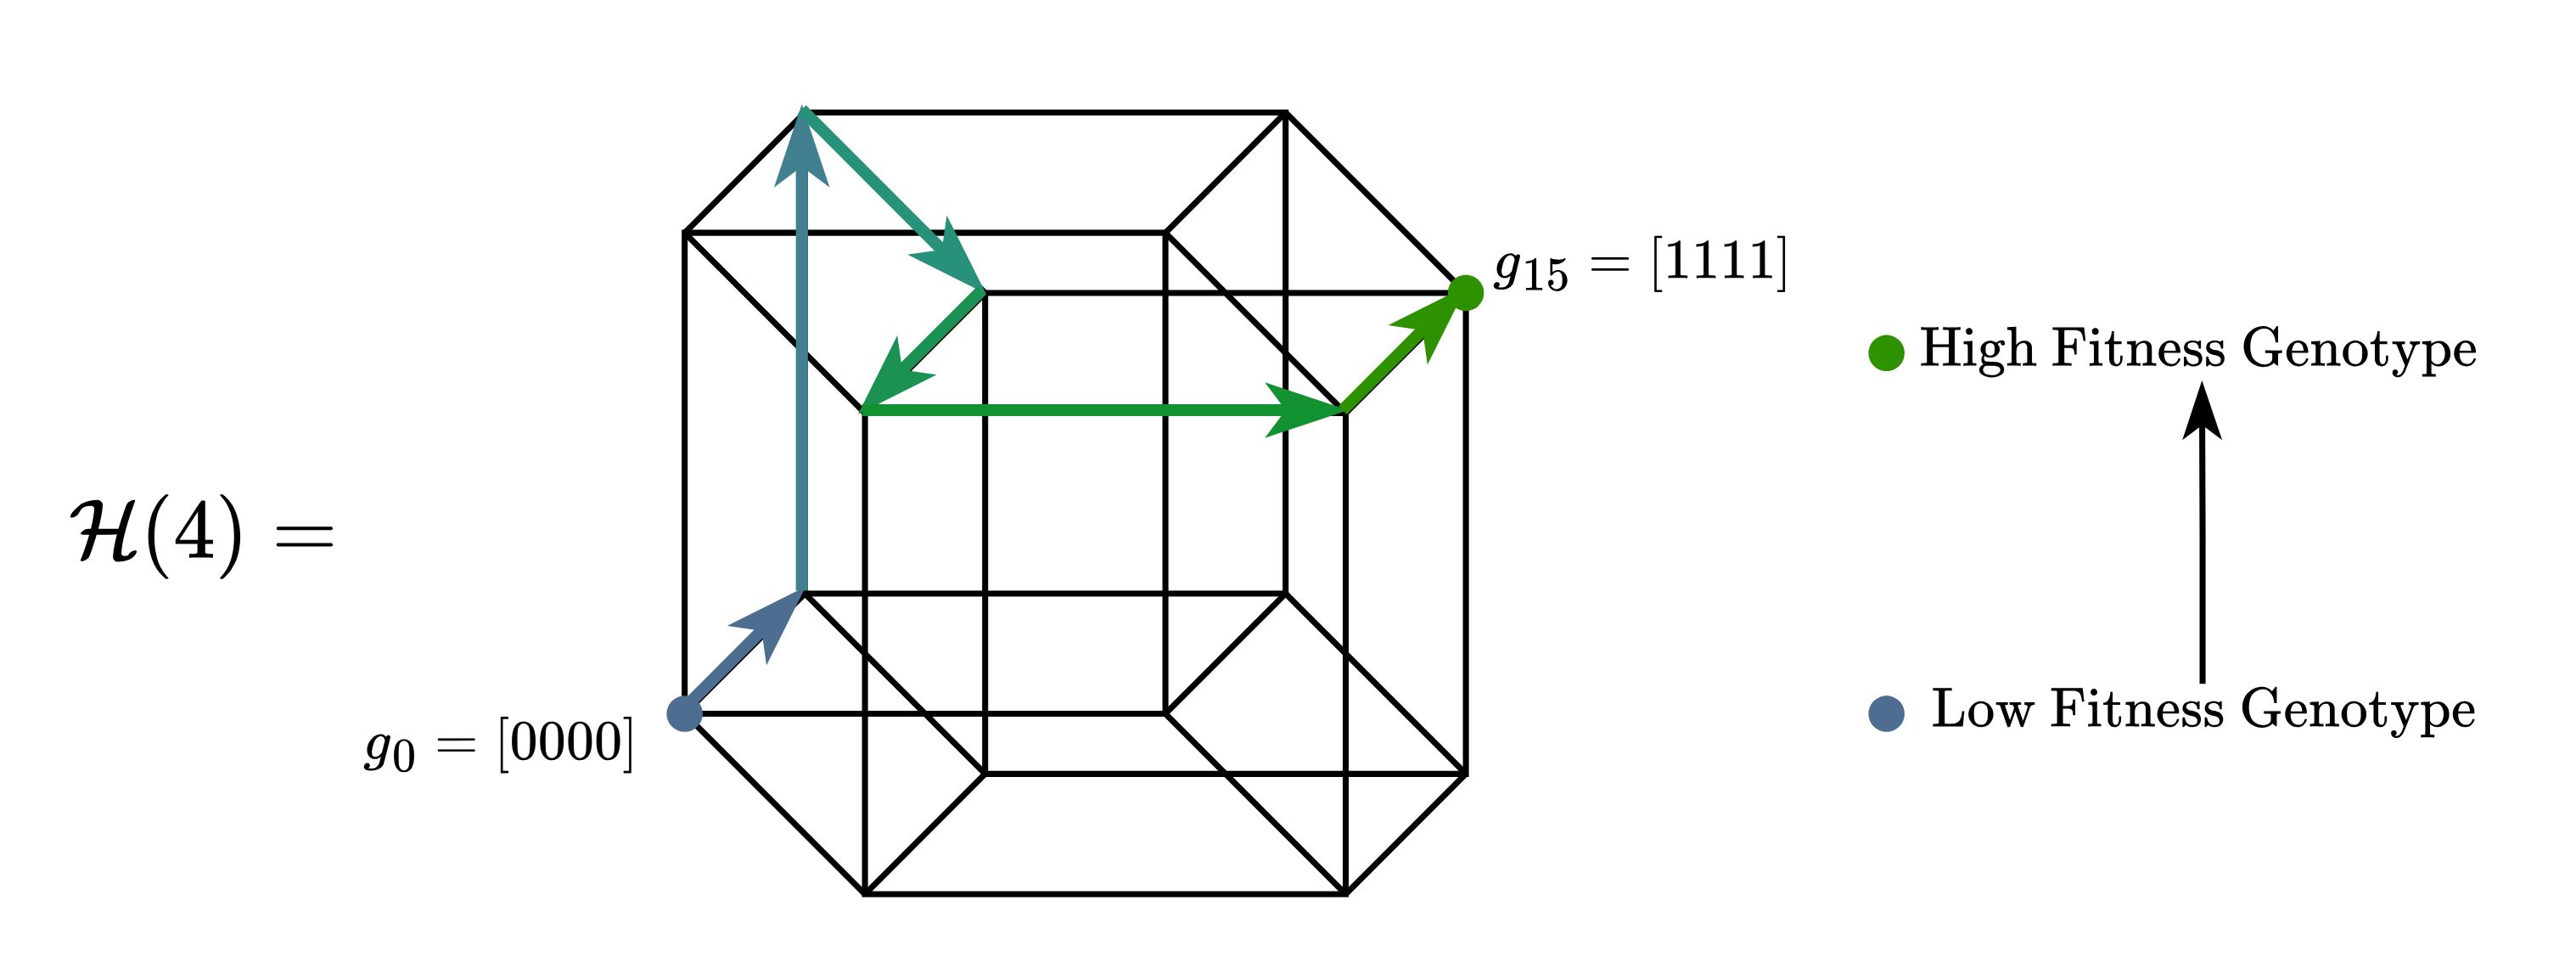
\includegraphics[width = 0.5\textwidth]{figures/simple_landscape.png}
	\caption{A 4-dimensional hypercube representing a 4-locus model. Genotypes are represented as binary strings e.g. [0000], and adapting populations generally traverse the landscape from low (blue) to high (green) fitness.}
	\label{genotype_space}
\end{figure}

The assignment of fitness values to genotypes entails sampling two probabilistically determined components: Locus-wise additive effects $A = (a_1, \cdots, a_i) \overset{iid}{\sim} \mathcal{N}(0, \sigma_a)$ are drawn from a normal distribution, and each genotype $g$ receives a unique epistatic component $e_g \sim \mathcal{N}(0, \sigma_e)$.  Fitness values for some arbitrary genotype can then be assigned as the sum of the product of the additive effects and the genotype, plus the epistatic component, as an exponential: 

$$f_g = \exp{\left(e_g + \sum_{i=0}^{L} a_i g_i\right)}$$

In this way, a 0 in the genotype represents a "neutral" allele, and 1 an allele with either a positive or negative effect. Epistasis is represented in the ratio between the variance of additive components and epistatic components, and we control its effect on the landscape by varying the epistatic $\sigma_e$ relative to $\sigma_a$ - in cases where the epistatic component is small the additive component dominates and the landscape becomes easily predictable, whereas when epistatic effects are large and outweigh the additive component, there is virtually no correlation between different genotypes and ruggedness is high. We proceed to model populations of individuals with different genotypes adapting on these landscapes through numerical simulations.

A discrete-generation RMF model with Wright-Fisher dynamics was implemented based on Li et al. 2024 \cite{liRapidAdaptationRecombining2024} and previous software \cite{amadoSTUNForwardtimeSimulation2023}. We model a static $N$ total individuals mutating and reproducing simultaneously in each generation, where each individual may be part of one of many subpopulations of genotypes $g$. To initialize the simulation, we specify the maximum number of loci in the model and consequently the length of the vector of additive effects to generate, the simulation length, the variance $\sigma_e$ of the epistatic component, and the mutation rate $\mu$ - the probability for an individual to generate a mutant of Hamming distance 1 from its parent. We proceed to instantiate subsequent generations by first generating mutants from each extant genotype with population $P$ through binomial sampling: $\text{Binomial}(n = P, p = \mu)$. We adjust the corresponding subpopulation counts for each genotype and calculate fitnesses for new genotypes if necessary, and then assign from $i$ extant genotypes for all individuals in the new generation of size $N$ new genotypes according to their relative fitness: $\text{Multinomial}(N, p^{\prime} = (p^{\prime}_1, \cdots, p^{\prime}_i))$ given $p^{\prime}_i = p_i * \frac{\omega_i}{\bar{\omega}}$, where $p_i$ is some genotype's current frequency, $\omega_i$ is its fitness, and $\bar{\omega}$ is the average fitness across all extant genotypes. Therefore, highly fit mutants gain an advantage during sampling and are less likely to be eliminated through drift. Simulations were generally run for 50000 generations before terminating.

\subsection*{Counter-Based Random Number Generation}

With this manner of simulation, the same genotype may arise and disappear multiple times due to drift - we then require the ability to reproducibly generate many unique epistatic components to calculate the fitness of any possible genotype on the landscape. We typically do this by mapping a sequence of random numbers in the state space of a pseudorandom number generator (PRNG) to base-10 genotypes, but as the size of genotype space grows large, retrieval in $O(n)$ time becomes unwieldy. Figure \ref{prng} shows the process of generating random numbers with a PRNG, where in order to generate the $i^{\text{th}}$ random number $r$ in a sequence, $i-1$ prior values must be calculated. To mitigate this problem, we utilize counter-based random number generators (CBRNGs), which can retrieve any number from the state space of the generator in constant time as a function of a seed number and an index (Figure \ref{cbrng}). In our implementation, the generation of random epistatic components was performed in Julia using an ARS1x generator \cite{JuliaRandomRandom123jl2024} of the Random123 package from D.E. Shaw Research \cite{salmonParallelRandomNumbers2011}, with a state space of $2^{128}$, this being the number of genotypes that can be modeled in a network.

\begin{figure}[h!]
	\centering
	\subfloat[\label{prng} PRNG]{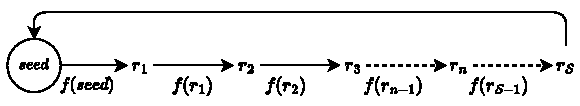
\includegraphics[width = 0.75\textwidth]{figures/prng.pdf}}
	\\
	\subfloat[\label{cbrng} CBRNG]{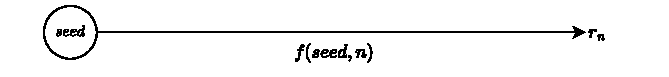
\includegraphics[width = 0.75\textwidth]{figures/cbrng.pdf}}
	\label{rngs}
	\caption{\textit{(a)} Scheme for a PRNG: each random number $r_i$ in the generator yields the next state $r_{i+1}$ through $f(r_i)$. Each random number $r_i$ is mapped to a base 2 number in genotype space based on its index $i$. Generators have a state space of $\mathcal{S}$ values, after which the values output will cycle back to the seed. \textit{(b)} Scheme for a CBRNG: Each state $r_i$ in the generator can be yielded in constant time from only the seed sequence and an index. These will also cycle, when inputting an index larger than $\mathcal{S}$.}
\end{figure}

\subsection*{A Model Extension for Genome Evolution}

The model as described above is static, and assumes all individuals have the same genome. To allow for selection to additionally act upon genome size changes, we extend the model to give individuals a genome $G$ and a genotype $g$ on that genome, and calculate fitness as a function of both. Each $G$ and $g$ are binary strings of the maximum possible length for the genome ($L_{\text{max}}$), and we utilize $G$ to determine which loci in $g$ may mutate: a 1 value in the genome represents the presence of a gene or functional genetic element, and allows the corresponding position in $g$ to be mutated between 0 and 1, while a 0 in $G$ ensures that position in $g$ will always be 0, and thus never contribute additively to fitness. Both mutational processes (genome and genotype mutation) are assigned their own mutation rate parameter ($M$ and $\mu$, respectively), and therefore to access the highest fitness states, populations must first select for genomic changes in $G$ that allow them to mutate their genotypes $g$ to those fitness peaks. Additionally, we assume that when new genes evolve, they may interact nonadditively with other previously existing genes, and thus genomic changes in $G$ must also be able to change the epistatic component, not only genotype $g$ changes: we therefore make the epistatic component $e_{G,g}$. As the CBRNG function takes both a seed and an index, we use the genome as a seed and the genotype as the index for to retrieve unique epistatic components for every combination of genome and genotype in 128-bit space. Effectively, we allow for individuals to navigate a network of landscapes of different sizes, simultaneously adapting on those landscapes and transitioning between them by changing their genomes.

\subsection*{Scripting}

All functions for the simulation of this model were written in a `Utils.jl` file. This includes methods for the generation of additive effects, the generation of mutants from a population, or the resampling of a population for a new generation. To allow for reproducibility, the model requires seeds for PRNGs that determine the initial genome and genotype, the additive effects vector, and the mutations made in each generation. In this way, rerunning a simulation with identical parameters but varying only the mutation seed allows us to simulate replicates on the same landscape and starting position, that may generate different mutants and thus different outcomes over the course of the simulation. Examinations of different classes of landscapes were then performed in separate scripts, each by defining different parameters for the model, and for each replicate, initializing the PRNGs with the appropriate seeds, and running the simulation function.

\section*{Results}

\subsection*{Additive Limit}

We examine first the simple case where $\sigma_{e}$ is zero and the values of the additive effects $a_i \neq 0$, resulting in a monopeaked landscape with no epistasis. Simulations were initialized with the following parameters, and 100 replicates were run by varying the seed value for the mutational rng.

\begin{center}
    \begin{tabular}{ | c | c | }
	\hline
	Maximum Size & 20 \\ \hline
	Initial Size & 1, 10, 20 \\ \hline
	Population & 1000 \\ \hline
	Generations & 50000 \\ \hline
	$\sigma_e$ & 0 \\ \hline
	A & $a_i \overset{iid}{\sim} N(\mu_a = 0, \sigma_a = 0.1)$ \\ \hline
	$\mu$  & 1e-4 \\ \hline
	$M$ & 1e-4 \\ \hline
    \end{tabular}
\end{center}

As there is no epistasis, populations will rapidly reach equilibrium at the fitness maximum on any individual landscape, whereas to find the global peak between all landscapes a slightly different behavior is observed. Since a mutation to $0$ in either the genotype or genome produces an identical fitness, on average $50\%$ of negative additive effects will be removed via each type of mutation, resulting in half of them being present on the genome with $G_i = 1, g_i = 0$, and half not present with $G_i = g_i = 0$. This balance will gradually fluctuate. Figure \ref{additivedynamics} shows genome sizes over time for starting genome sizes 1, 10, and 20 for one replicate with 10 positive additive effects. 

\begin{figure}[h!]
	\centering
	\subfloat[\label{ad:sub1} Initial genome size 1]{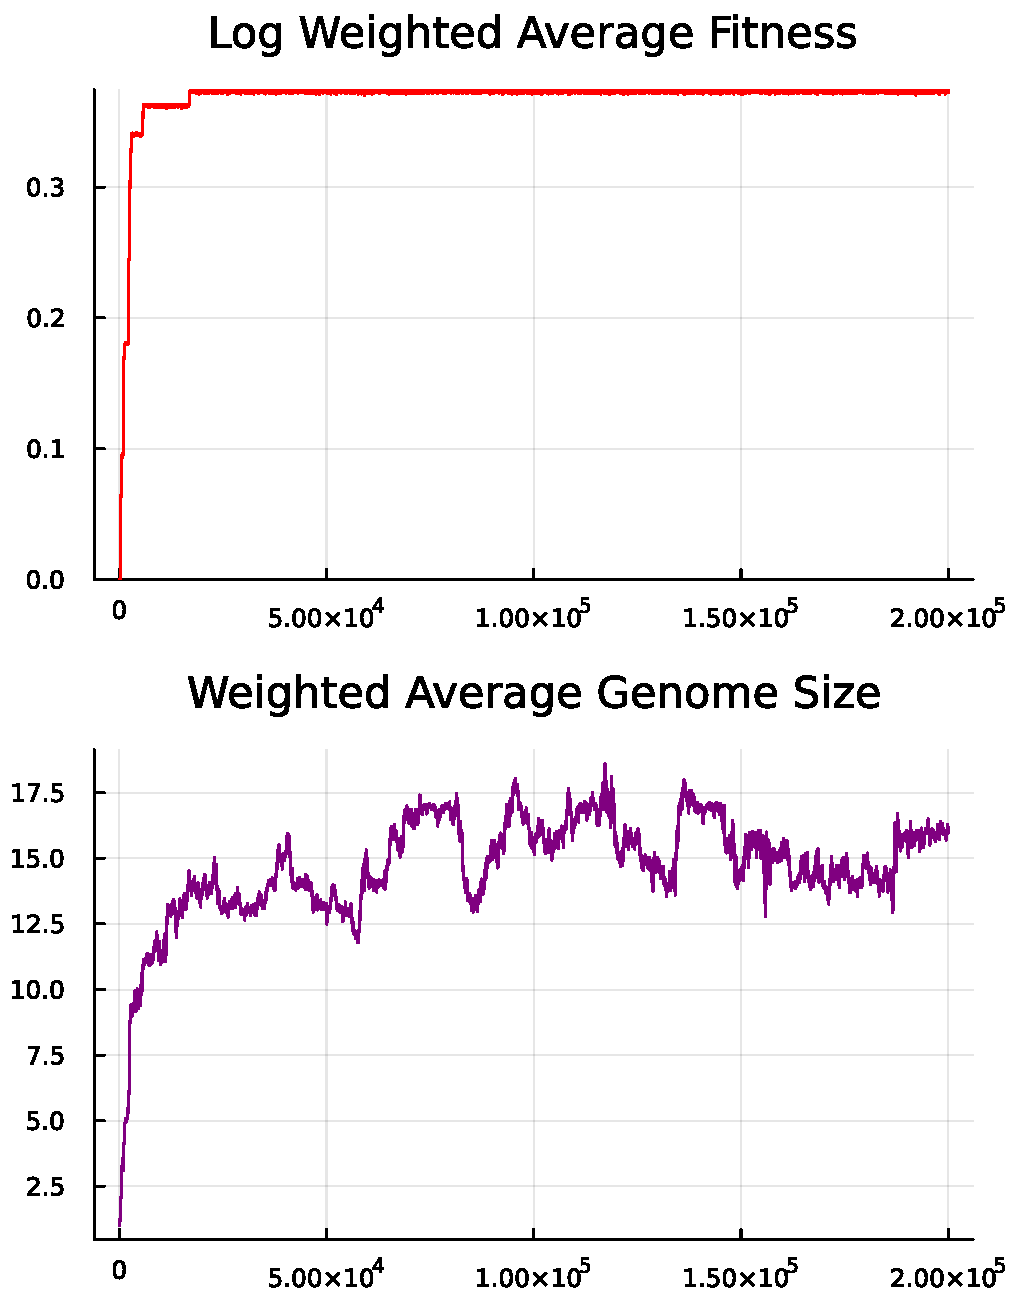
\includegraphics[width = 0.33\textwidth]{figures/L20l1i1_20250902_1035.pdf}}
	\subfloat[\label{ad:sub2} Initial genome size 10]{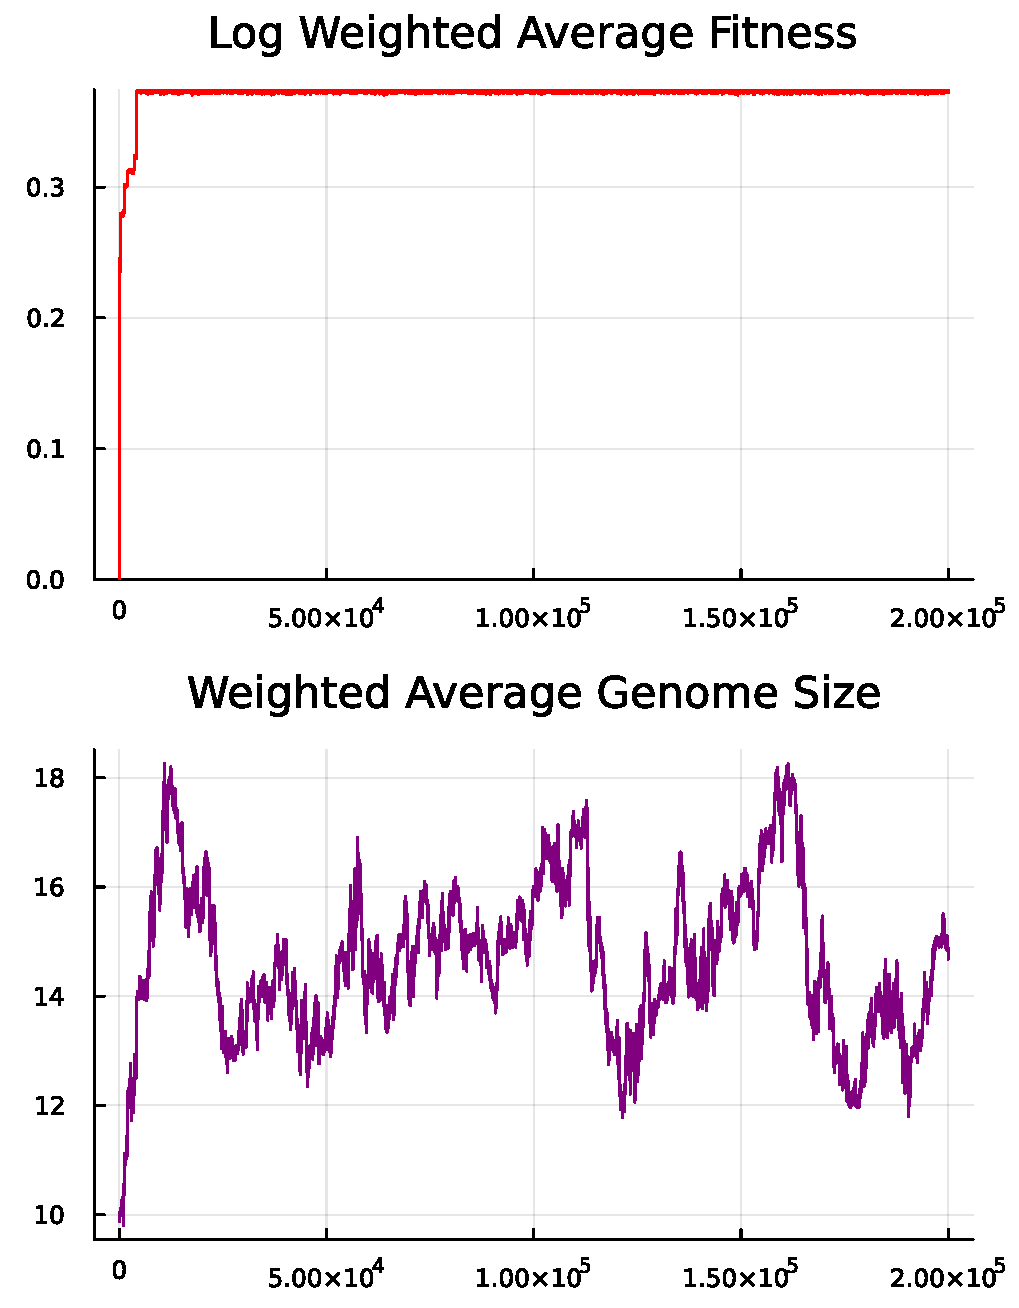
\includegraphics[width = 0.33\textwidth]{figures/L20l10i1_20250902_1035.pdf}}
	\\
	\subfloat[\label{ad:sub3} Initial genome size 20]{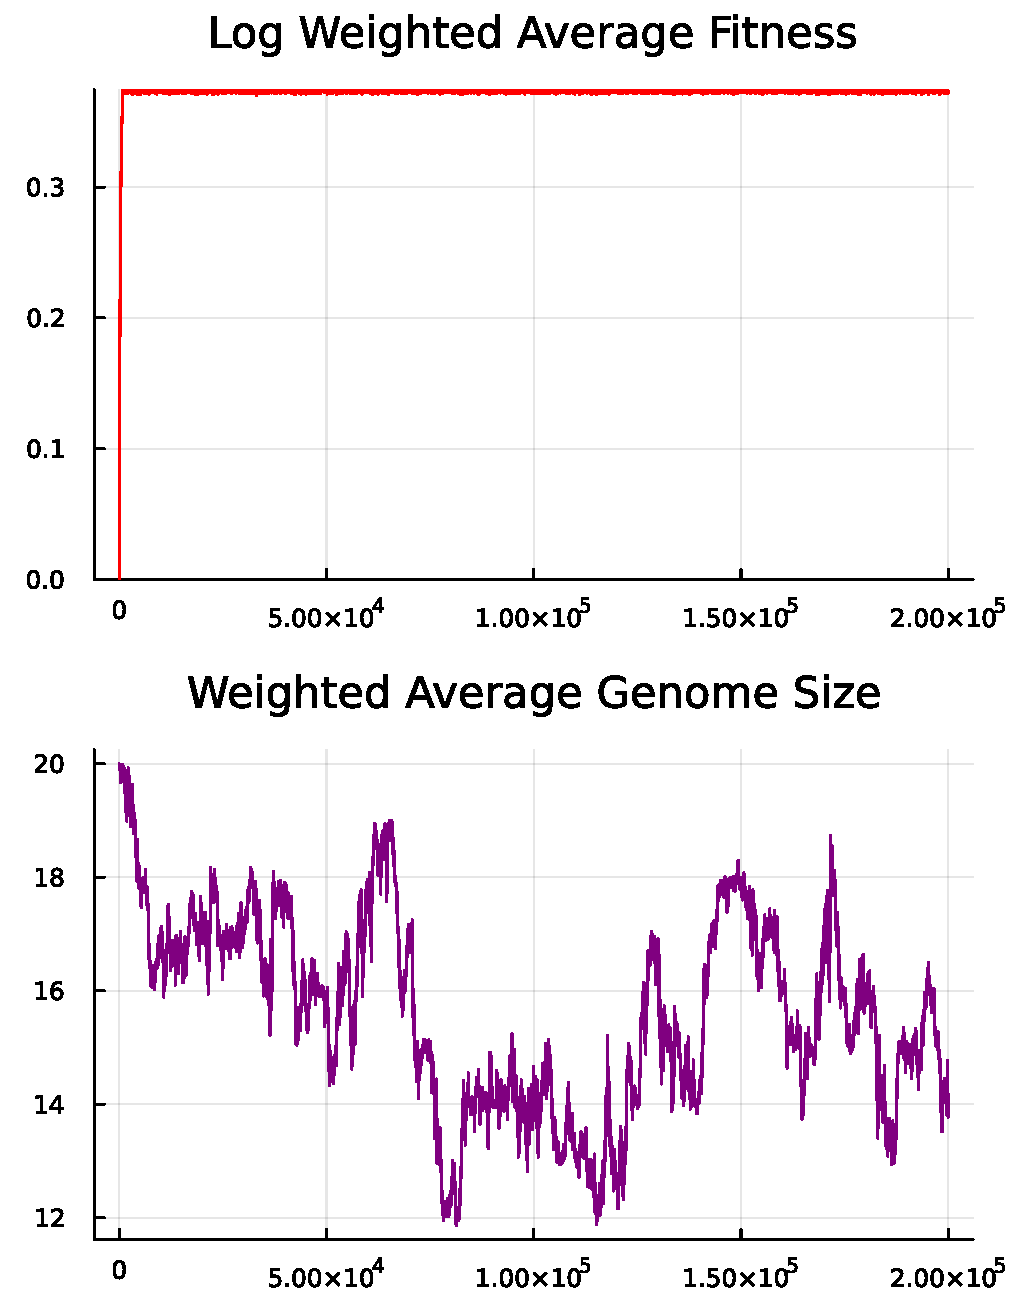
\includegraphics[width = 0.33\textwidth]{figures/L20l20i1_20250902_1035.pdf}}
	\subfloat[\label{ad:sub4} Densities of genome size time series]{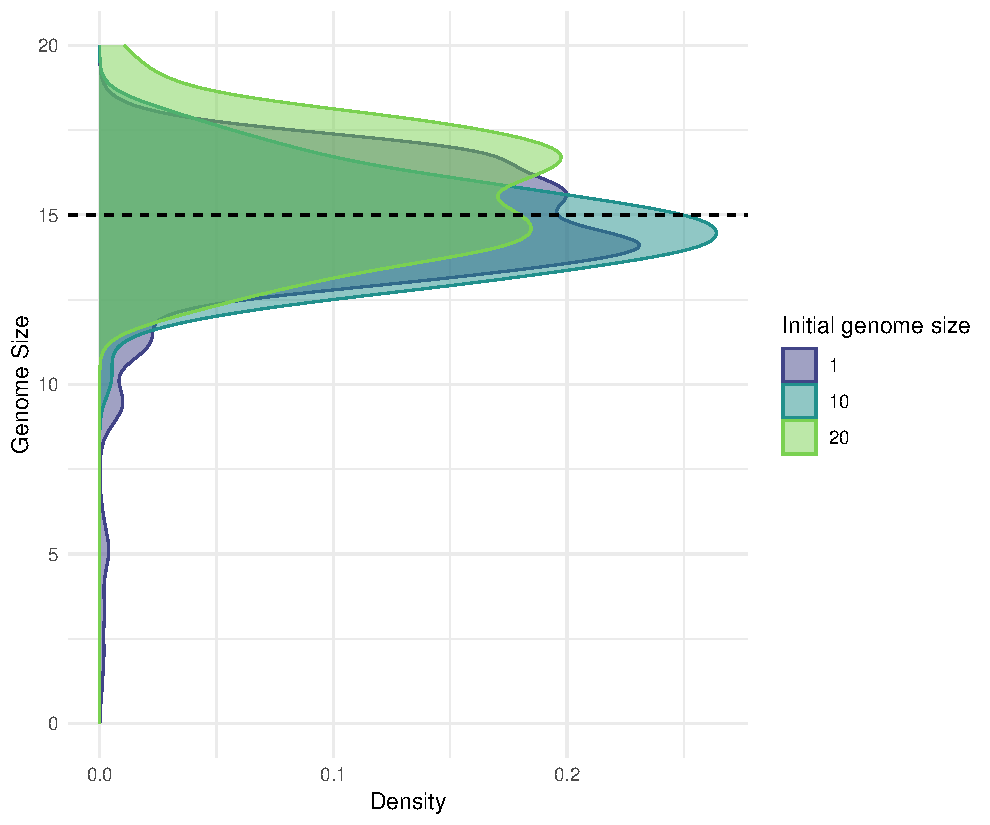
\includegraphics[width = 0.33\textwidth]{figures/random_walk_additive.pdf}}
	\caption{\textit{(a), (b), (c)}: Time series of genome size and fitness for example simulations starting at 1, 10, and 20 loci. \textit{(d)}: densities of genome size time series all form a mean around 15.}
	\label{additivedynamics}
\end{figure}

It can be observed that fitness reaches the same value and plateaus in all three cases within relatively few generations, while genome size simultaneously moves to and thereafter fluctuates about 75\% of the maximum. This can be attributed to the random swapping of the two fitness-equivalent mutations as described above, while maintaining a $1$ state for all positive effects. In this instance, the 10 positive additive effects will always be $G_i = g_i = 1$, and on average, out of the remaining ten negative additive effects, five will be not present in the genome ($G_i = g_i = 0$), while five will be and mutated to a $0$ state ($G_i = 1, g_i = 0$), resulting in a mean genome size of 15 averaged over the entire time series (Figure \ref{ad:sub4}). We can see how, in the complete absence of epistasis, there are many landscapes that produce equivalent optimal fitness and as such there is no single equilibrium point, and that populations are not constrained from reaching these fitness-optimal states by their starting genome size. 

\subsection*{Uncorrelated Limit}

We next investigate uncorrelated (known alternatively as House of Cards) landscapes, where all additive effects $a_i = 0$ and $\sigma_e$ is positive. This produces maximally rugged landscapes under the RMF model, where each genotype on a landscape and each landscape in genome space has a randomly drawn fitness and is uncorrelated to any other. We simulated 200 replicates under the following conditions:

\begin{center}
    \begin{tabular}{ | c | c | c | }
        \hline
	Maximum Size & 20 & 100 \\ \hline
	Initial Size & 1, 5, 10, 15, 20 & 1, 25, 50, 75, 100 \\ \hline
	Population & 1000 & " \\ \hline
	Generations & 50000 & " \\ \hline
	$\sigma_e$ & 1 & " \\ \hline
	$A$ & All $a_i = 0$ & " \\ \hline
	$\mu$  & 1e-4 & " \\ \hline
	$M$ & 1e-4 & " \\ \hline
    \end{tabular}
\end{center}

As fitnesses are determined solely through the sampling of the epistatic component distribution $e_{G,g}$, larger landscapes will tend to have higher fitness peaks overall, due to a greater number of samples producing, on average, more extreme values. This effect can be shown analytically in the expectation of the distribution of fitness peaks, as determined through extreme value theory:  $$\mathbb{E}[X] = \exp{\left(\sqrt{2L \ast (\frac{L \ast \sigma_a^2}{2} + \sigma_e^2) \ast \ln(2)}\right)}$$ Given a constant variance of additive and epistatic terms between landscapes, the mean value of fitness peaks increases with the number of loci as an exponent of $e$, either sub- or superlinearly depending on parameters (Supplementary figure \ref{supp:peak_scaling}). We see this confirmed in Figures \ref{ul:sub1} - \ref{ul:sub3}, where in both static (genome mutation parameter $M = 0$) and expanding ($M < 0$) landscape cases, an increased starting number of loci leads on average to higher fitness values. We also observe when comparing initial genome size 1 between expanding landscapes with $L_{\text{max}}$ of 20 and 100, that final fitnesses also scale with maximum size. However, final genome sizes do not appear to reach these sizes associated with higher fitness maxima; they are instead highly correlated with initial size. Figures \ref{ul:sub4} and \ref{ul:sub5} visualize the distributions of final genome sizes by initial size, wherein genome sizes end in a relatively compact distribution not far from the initial size. These distributions appear to skew in the direction of half the maximum genome size, and the magnitude of such remains constant as the number of loci increases. At the extremal case of $L_{\text{initial}} = 1$, for both $L_{\text{max}} = 20$ and $L_{\text{max}} = 100$ the skew of the final size distribution is around 5, and correspondingly for test cases at $^1/_4$, $^1/_2$, and $^3/_4$ of the maximum genome size the skew is proportionally similar regardless of $L_{\text{max}}$. This effect appears to be a mutational bias from the genome size limit, where smaller genomes that mutate are by chance more likely to change a 0 in their genome to a 1, and conversely a large genome with many 1s is more likely to reduce its genome size by changing to a 0. We conclude that larger genomes will have higher fitness outcomes on average, yet see that on landscapes with epistasis populations do not indefinitely increase their genome size - there is a finite skew to the final sizes that constrains achievable fitness.

\begin{figure}[h!]
	\centering
	\subfloat[\label{ul:sub1} Final fitnesses:\\ Static landscapes]{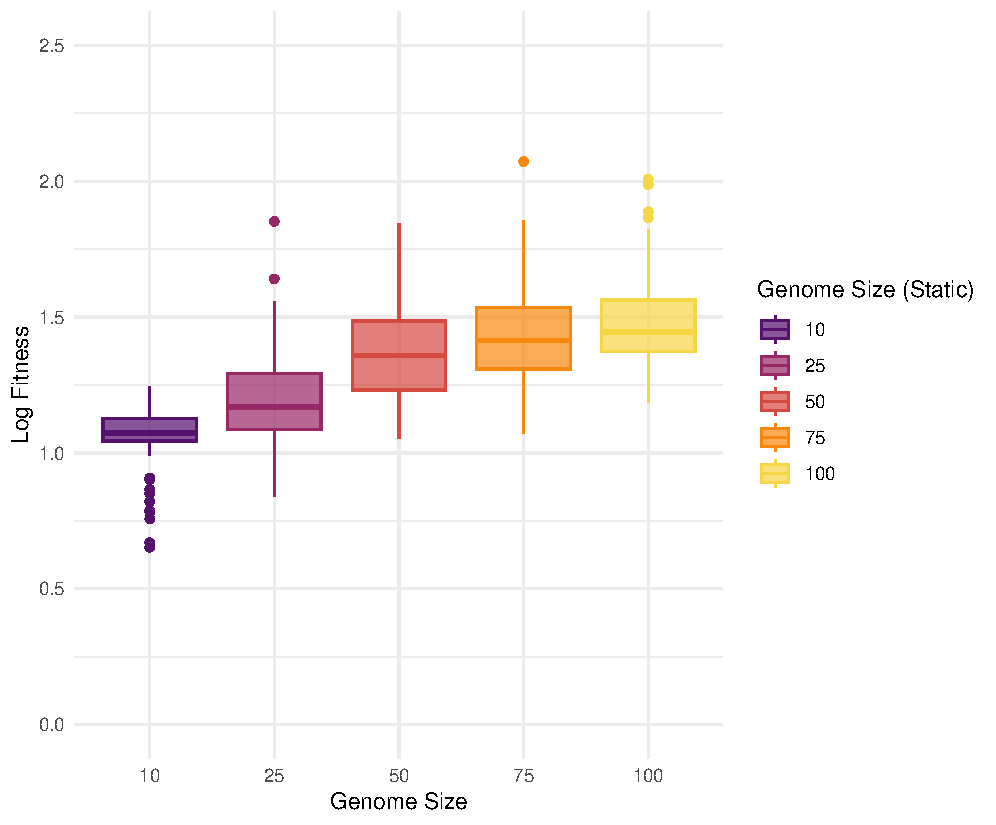
\includegraphics[width = 0.333\textwidth]{figures/05-2_static_finalfitness.pdf}}
	\subfloat[\label{ul:sub2} Final fitnesses:\\ Expanding landscapes \\($L_{\text{max}} = 20$)]{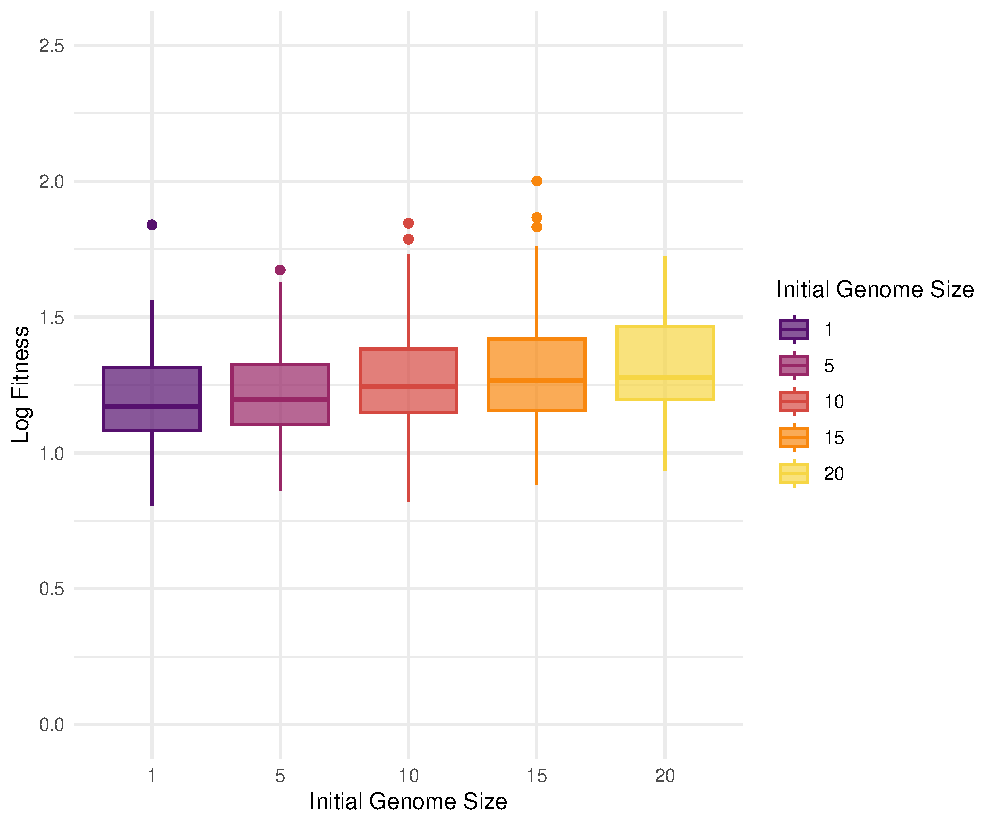
\includegraphics[width = 0.333\textwidth]{figures/06-1_expanding_initialsize_fitness.pdf}}
	\subfloat[\label{ul:sub3} Final fitnesses:\\ Expanding landscapes \\($L_{\text{max}} = 100$)]{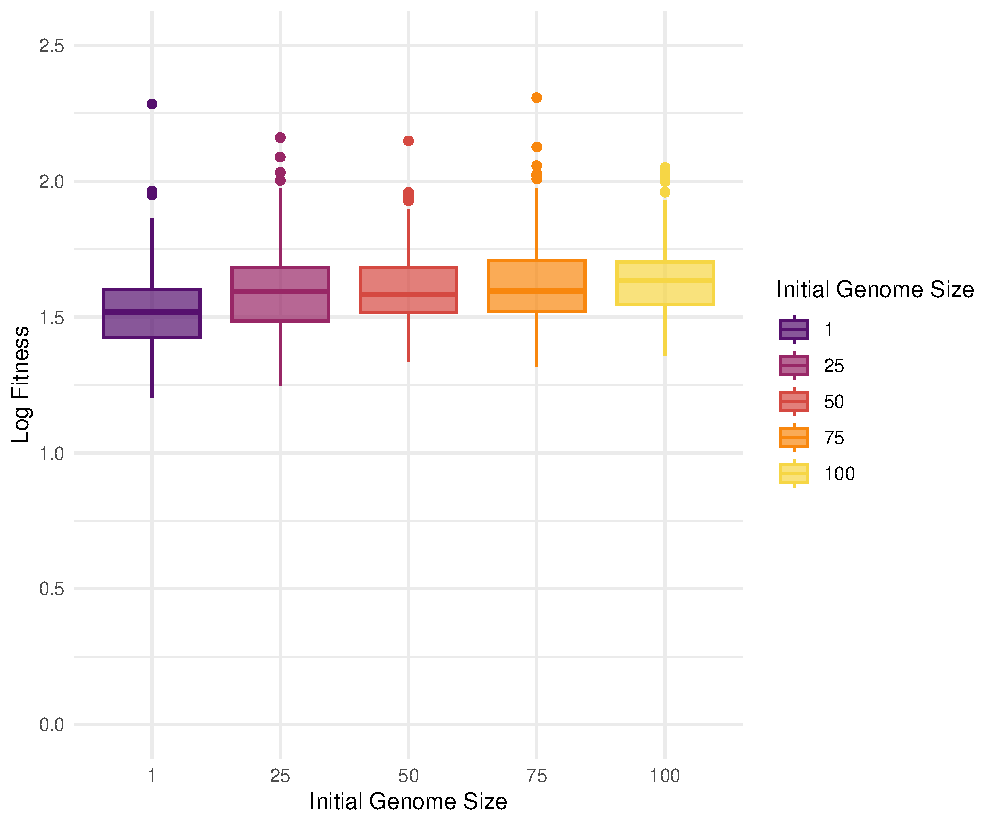
\includegraphics[width = 0.333\textwidth]{figures/06-4_expanding_initialsizefitness_2.pdf}} \\
	\subfloat[\label{ul:sub4} Final size distributions \\($L_{\text{max}} = 20$)]{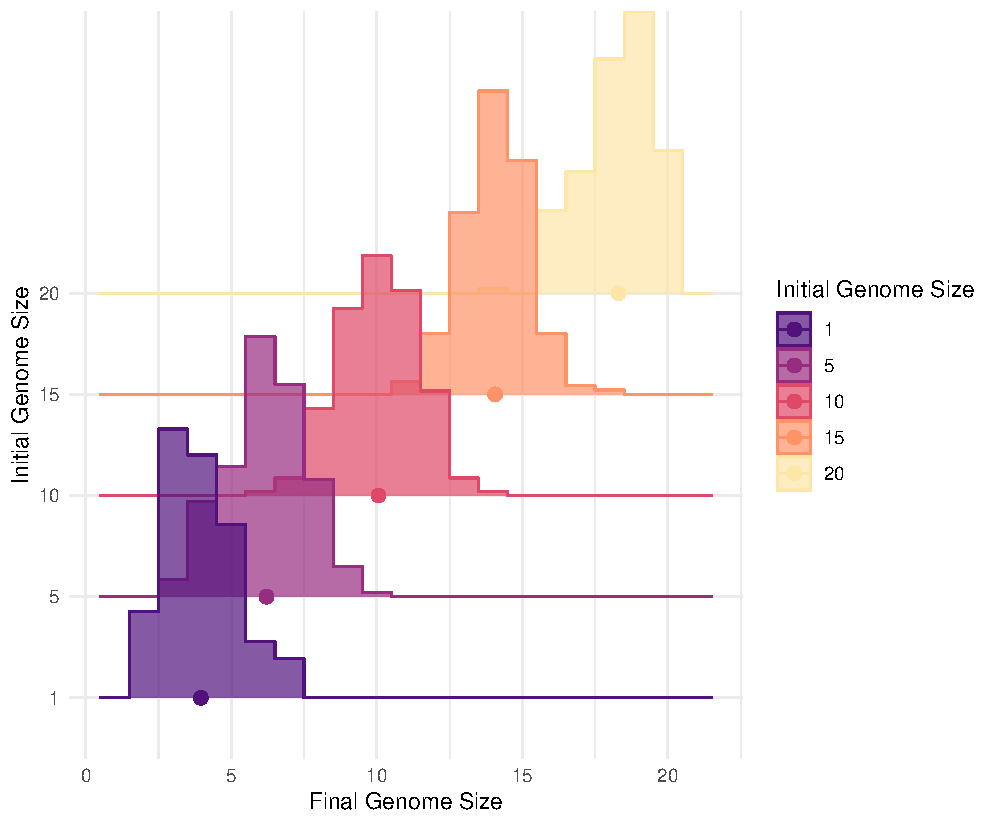
\includegraphics[width = 0.333\textwidth]{figures/06-3_expanding_initialfinalsize.pdf}}
	\subfloat[\label{ul:sub5} Final size distributions \\($L_{\text{max}} = 100$)]{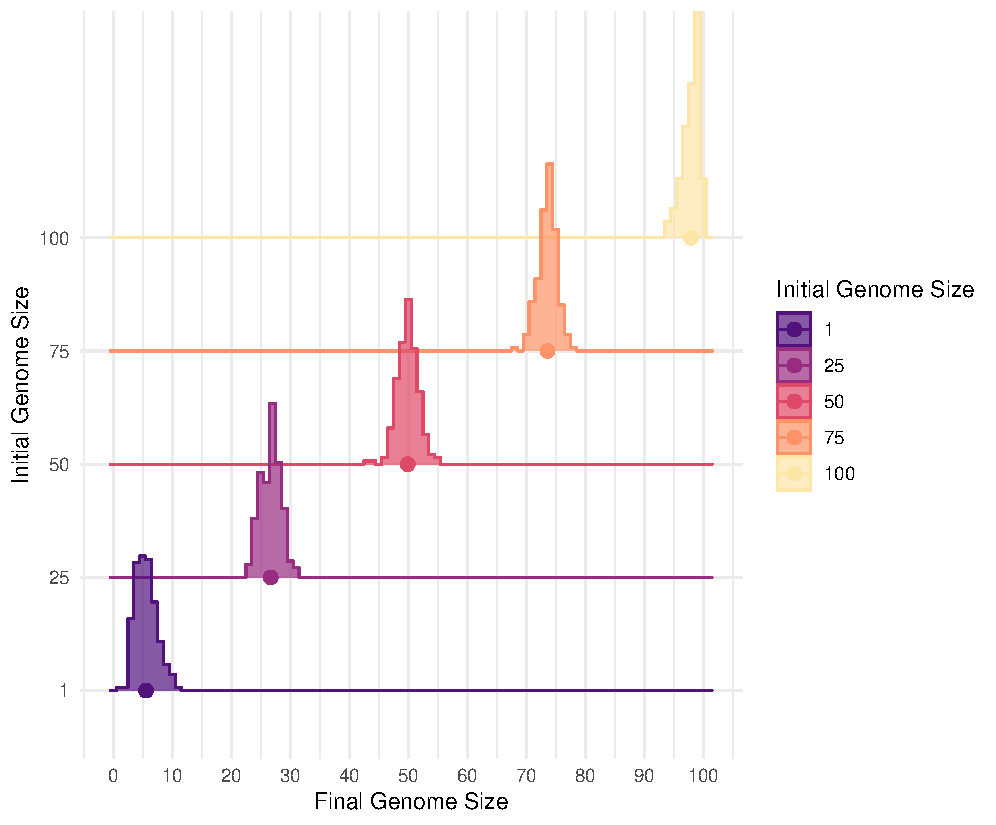
\includegraphics[width = 0.333\textwidth]{figures/06-6_initialfinalsize_2.pdf}}
	\caption{Final fitnesses of \textit{(a)} static and \textit{(b),(c)} expanding landscapes, \textit{(d),(e)} final sizes of expanding landscapes.}
	\label{uncorrelated_fitnesses}
\end{figure}

\pagebreak

\subsection*{Intermediate Epistasis}

We last turn to rugged landscapes with both additive and epistatic components, which are most similar to empirical landscapes. We ran 5000 replicates of simulations with the following parameters:

\begin{center}
    \begin{tabular}{ | c | c | }
	\hline
	Maximum Size & 20 \\ \hline
	Initial Size & 5 \\ \hline
	Population & 1000 \\ \hline
	Generations & 50000 \\ \hline
	$\sigma_e$ & 0.1 \\ \hline
	$A$ &  $a_i \overset{iid}{\sim} N(\mu_a = 0, \sigma_a = 0.1)$ \\ \hline
	$\mu$  & 1e-4 \\ \hline
	$M$ & 1e-5 \\ \hline
    \end{tabular}
\end{center}

By setting the genome mutation rate $M$ an order of magnitude less than the genotype mutation rate $\mu$, we separate the time scales on which peaks on a landscape and transitions between landscapes are navigated to, allowing fitness peaks to be reached on each landscape before genome mutations are made. We track the genomic trajectories of these simulations over time, observing which final genome sizes are achieved, and the fitness peaks reached on each intermediate landscape along the way. 

Figure \ref{ie:sub1} visualizes the genome size trajectories of all simulations as they increase from an initial size of five until the end of the simulation. To simplify the plots, we remove replicates that do not have a monotonically increasing genome size, although the effect in these cases is consistent with the rest of the data (Supplementary figure \ref{uf}). We observe that although populations must not necessarily take fitness increasing paths to reach a peak on any given landscape, when transitioning between landscapes there does seem to be consistent fitness increases. Additionally, replicates that are able to increase their genome size seem to occupy lower fitness regions of each landscape, as opposed to those that end the simulation at some landscape size, which tend to have higher fitness - this behavior is further examined in figure \ref{ie:sub2}. Here we see the distributions of fitness values at each genome size split between those replicates which ended the simulation at that size, versus those that continued to expand their genome. Consistently among all genome sizes, we notice that replicates that increase their genome size past some size actually have, on average, lower fitnesses than those that do not. This implies that populations that begin less fit on some landscape and who minimize their fitness gain on each subsequent landscape possess a greater ability to expand their genome. When comparing with figure \ref{ie:sub4}, which displays the same but for uncorrelated landscapes, the magnitude of difference is greater but the fitness values are lower. This is in alignment with expected effect of epistasis, which will create more, lower fitness peaks on a landscape, such that it is more likely that populations will become stuck at them. Finally, we can confirm in figure \ref{ie:sub3} that the times in which genome size transitions are made is quite similar between those at endpoint at some genome size, and those that continue to expand, suggesting, at least, that genome size transitions are not happening \textit{before} a local maximum is reached on a landscape. 

\begin{figure}[h!]
        \centering                                                                                                                                                  \subfloat[\label{ie:sub1} Fitness trajectories]{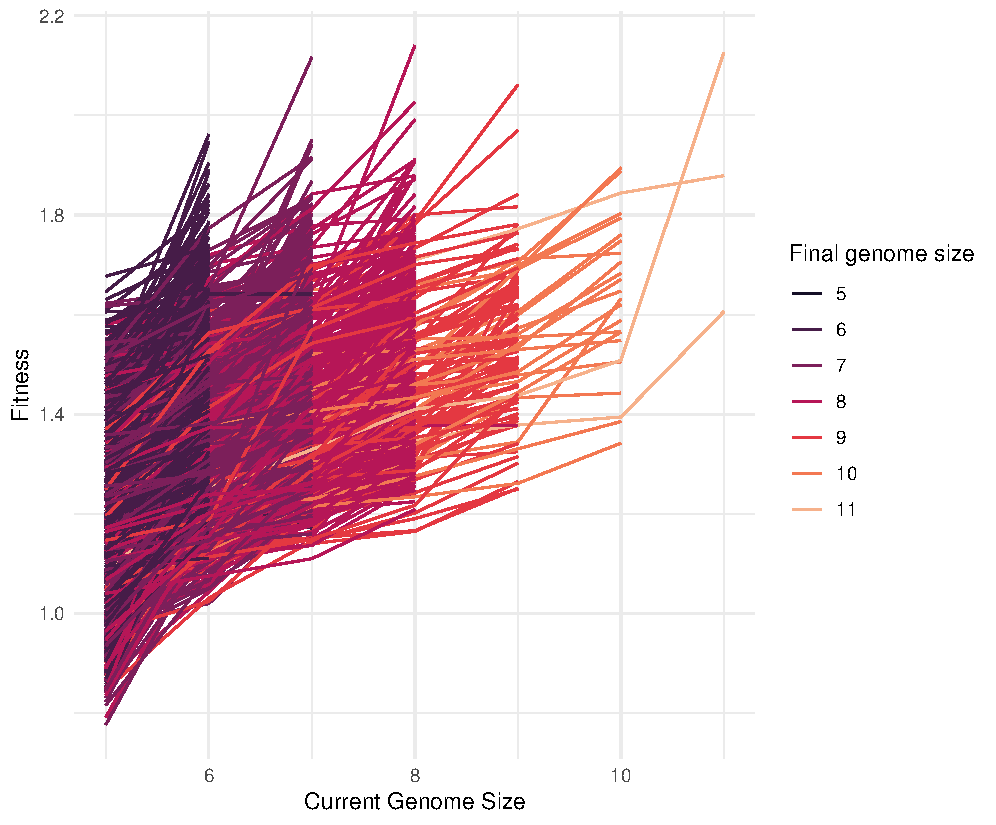
\includegraphics[width = 0.4\textwidth]{figures/genome_trajectories.pdf}}
        \subfloat[\label{ie:sub2} Endpoints]{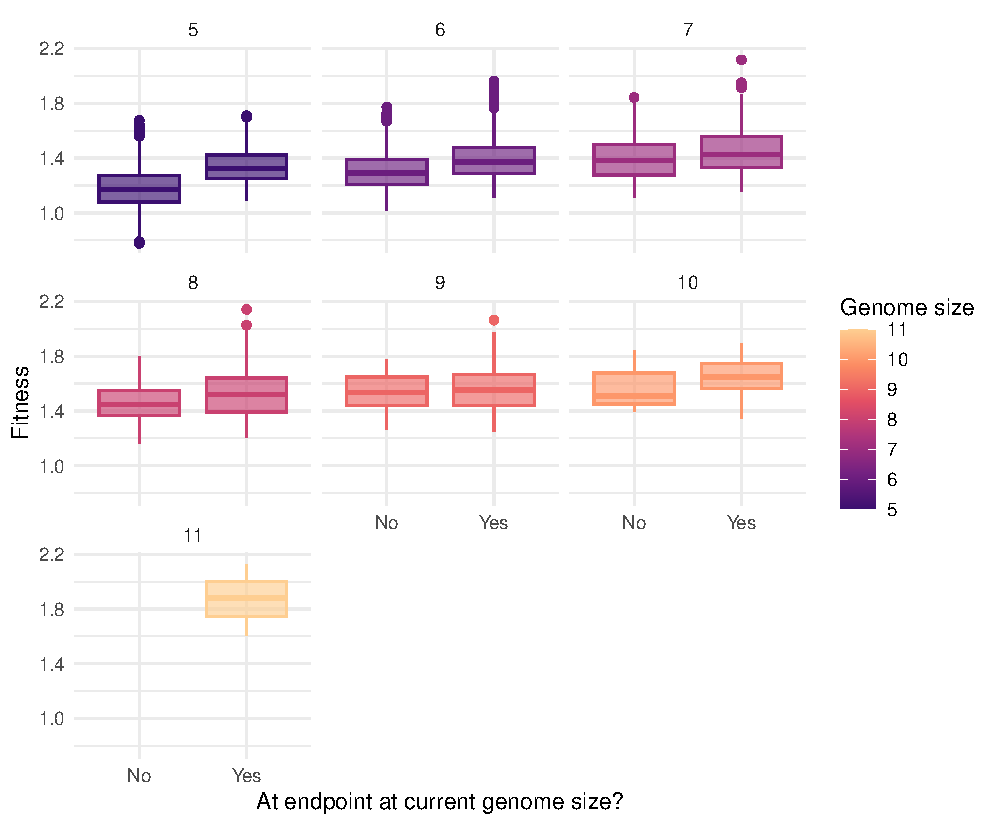
\includegraphics[width = 0.4\textwidth]{figures/endpoint_boxplots.pdf}} \\                                             \subfloat[\label{ie:sub3} Size transition timings]{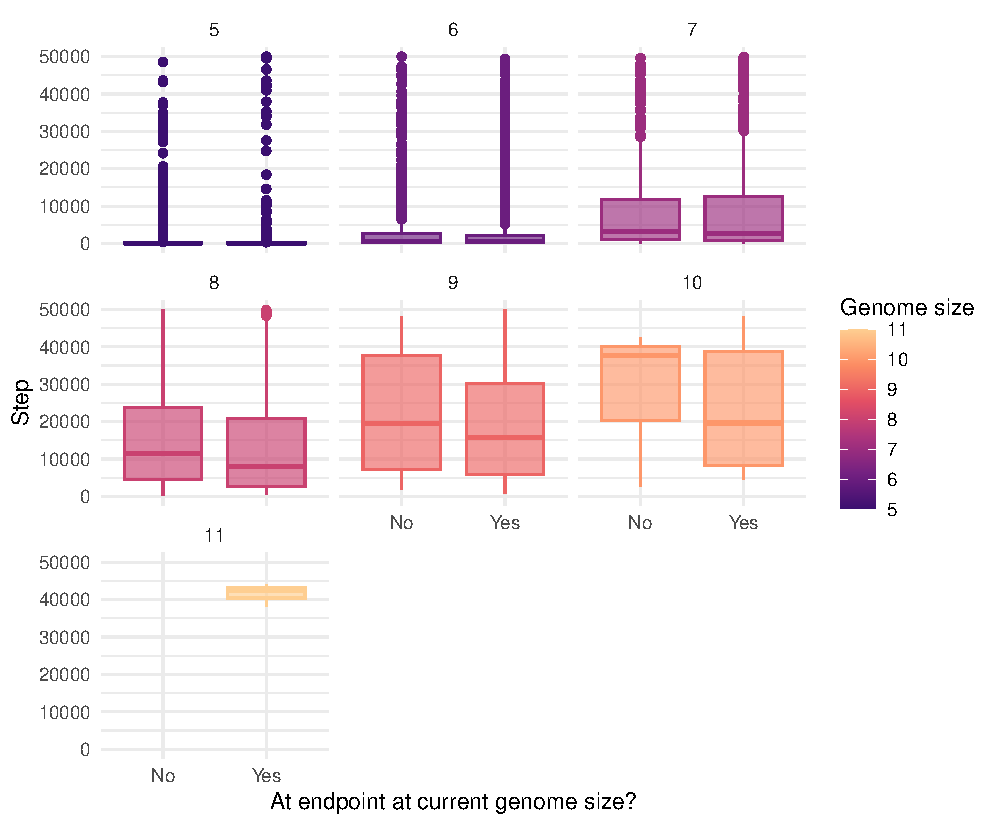
\includegraphics[width = 0.4\textwidth]{figures/timings.pdf}}                                            \subfloat[\label{ie:sub4} Endpoint comparisons on uncorrelated landscapes.]{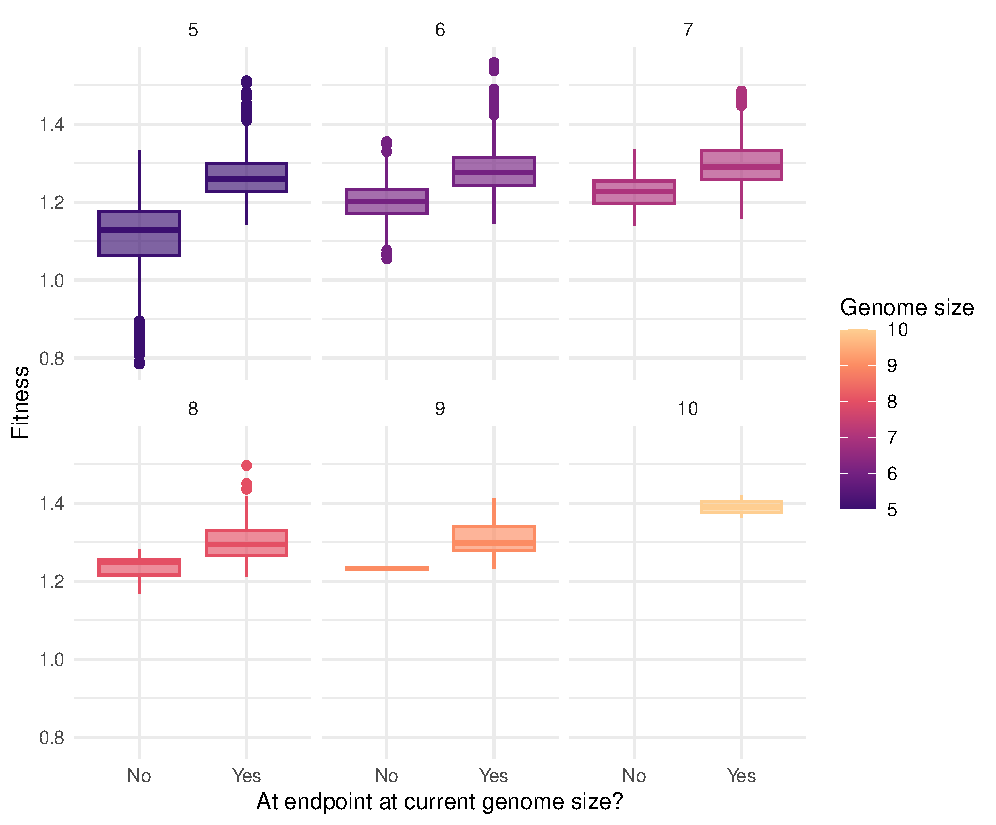
\includegraphics[width = 0.4\textwidth]{figures/hoc_boxplots.pdf}}              \caption{\textit{(a)}: Fitness trajectories over different genome sizes, for replicates with monotonically increasing genome size \textit{(b)}: fitness comparisons of endpoint and non-endpoint simulations at various genome sizes, \textit{(c)}: Distributions of generation times at which genome size transitions are made, \textit{(d)}: fitness comparisons as in \textit{(b)} on uncorrelated landscapes}
        \label{intermediate_epistasis}
\end{figure}

\pagebreak

\section*{Discussion}

The results of our simulations reveal some of the new dynamics we observe on expanding landscapes. We see how epistasis not only constrains navigability on individual landscapes, but the ability to transition between them as well. With additive landscapes, populations easily accumulate all possible additive effects regardless of starting genome size, whereas when epistasis increases, we see an increased amount of correlation between the starting and ending sizes. Most interestingly, we see what happens regarding adaptation over multiple landscapes with some amount of epistasis: populations that start from lower fitness and minimize fitness gain when increasing genome size end up with overall higher fitnesses. We believe this is due to an interaction between the scaling of the fitness landscape peak distribution and adaptability as fitness increases. As an individual gets fitter, the probability that any mutant will yield a fitness increasing path decreases, and this also extends to transitions between landscapes as well. Therefore adapting to a higher fitness peak on any given landscape actually decreases the probability to be able to increase genome size. However, we also know from examining final fitnesses achieved on larger landscapes, that the mean of the distribution increases because there are more states in genotype space, and therefore more extreme fitnesses have the potential to be generated. We can then state these two things succinctly:
	\begin{enumerate}
		\item Larger genome size results on average in higher fitnesses. 
	
		\item Higher fitness reduces ability to increase genome size.
	\end{enumerate}
These contradictory objectives in the context of epistasis result in the behavior that we see. Assuming a low enough genome mutation rate, fitness peaks will be reached in the current landscape before landscapes will change. Thus, populations that reach lower fitness peaks on a landscape, have a greater ability to increase their genome size, and therefore have a higher end probability to eventually achieve higher fitnesses, while never having a particularly high fitness (relative to other paths) over the course of the system's evolution. 

\subsection*{A model for the evolution of metabolism}

This is very intriguing. It suggests that systems that optimize and encode heritable information can actually benefit from avoiding high fitness states too early in the evolution of the system, and finds itself in concordance with results from a similar long-term evolution experiment \cite{woodsSecondOrderSelectionEvolvability2011}. To illustrate a biologically relevant process where our findings would apply, we here introduce a toy model for the evolution of a metabolic network. 

\begin{figure}[h!]
	\centering
	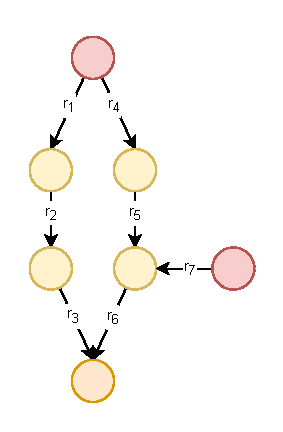
\includegraphics[width = 0.33\textwidth]{figures/evolving_metabolism.pdf}
	\caption{Example biochemical network space for a genome of maximum size 7.}
	\label{evomet}
\end{figure}

Here we represent chemical species as nodes and enzymatic reactions ($r_1\cdots r_i$) as edges with catalytic rate weights ($w_1 \cdots w_i$), and a genome can be comprised of any combination of genes for these enzymes. As shown in Figure \ref{evomet}, a typical cell will take nutrients (red, source nodes), and metabolize them through a series of biochemical intermediates (yellow nodes) to growth metabolites (orange, sink nodes) that cell requires to grow and divide, such as amino acids, nucleotides, or phospholipids. We therefore consider a metabolically viable cell to be one that has genes in its genome that construct at least one unbroken path between a source node and sink node. Fitness (or flux) calculations for larger, more empirical network models are typically done via flux balance analysis, \cite{orthWhatFluxBalance2010} but we will instead assume that the fitness for some genome is similar to that of the RMF model: $$f_G = e_G + \displaystyle\sum_{i=0}^{L}r_i w_i $$ That is, fitness is the sum of all weights $w_i$ for reactions of enzymes present in the genome plus an epistatic term $e_g$ to allow for tunable nonadditivity of a particular reaction set, with one additional rule: only reactions which lie directly on a source-sink path contribute to fitness. Like in the RMF model, we can then sample $e_G$ from $X \overset{iid}{\sim} \mathcal{N}(\mu, \sigma)$ and weights $w_i$ from a distribution with support between 0 and infinity such as a gamma, exponential, or absolute-value normal, as we assume enzyme rates in this context are generally not negative, nor catalytically bidirectional. 

This creates for us a rugged landscape with fitness maxima, or metabolically viable subnetworks, determined by the topology of the biochemical space chosen. We will not examine the consequences of random topologies on the outcomes of this model, but focus on how simply one trivially determined topology can produce behavior consistent with the previous results on expanding landscapes. At initiation, a genome size of three is the first point at which there are multiple viable genomes, encoding two different pathways for the metabolism of some nutrient - in this example, they can be represented as $1110000$ (or a reaction set of $[r_1, r_2, r_3]$) and $0001110$ ($[r_4, r_5, r_6]$). This is already quite common in bacterial physiology, where for example certain species may use the Embden-Meyerhof-Parnas \cite{sanchez-pascualaRefactoringEmbdenMeyerhof2017} or the Entner-Doudoroff \cite{conwayEntnerDoudoroffPathwayHistory1992} glycolysis pathways to produce the same products. All other factors equal, each pathway will have higher fitness in half of all cases, with the magnitude of the difference between the two a function of the variance of additive and epistatic components, and the current genome size. Then, upon expansion of the genome, one pathway immediately gains access to another nutrient, while the other must take a longer path in order to access the same - this may be something present in the environment that had been underutilized, and represents niche expansion. On a purely additive landscape, this is no problem for either starting point. Since the optimal solution is to possess all genes in metabolic space and adding them is neutral, so we would see both starting points expand their genomes to the maximum size, similarly to how the additive expanding landscapes were all able to reach the optimal equilibrium size. However, once introducing epistasis, the ability to add genes is constrained by the probability the the epistatic component increases with every consecutive genome expansion, and the greater it is at the beginning, or the larger the number of genes to add to complete a pathway, the less likely this is to be the case. Provided that the variance of reaction weights is sufficiently low relative to their mean, this will commonly cause the lower fitness variant at size three to gain higher fitness at size four, while the alternative pathway will likely not be able to expand its genome to also utilize the new resource. This also echoes the behavior seen on the expanding landscape models - through the evolution of the system to larger sizes, epistasis begins to constrain free genome expansion, making it instead highly contingent on initial size, and additionally gives an advantage to lower fitness variants to expand their genomes. 

In this work we show a new RMF model that incorporates a less frequently modeled part of evolution: that the genome can fluctuate in not only allele content but also in size, and that the behavior seen in this expanded model is not a simple recapitulation of a simpler fitness landscape. The dynamics observed demonstrate that lower-fitness but more evolvable genomes can achieve the highest fitnesses through genome evolution. Despite longer-term adaptational potential, a high strength of selection, especially in larger populations, make these trajectories less likely to survive in a Darwinian environment. Therefore, we hypothesize that a non-negligible amount of the particular forms life takes now can be attributed to these sort of contingencies: that highly successful adaptation in earlier environments has, in some cases, limited subsequent evolutionary innovation. We hope that these findings, and the model itself, allow researchers to generate more informed hypotheses about long-term genome evolution and help connect empirical findings to create a greater, more cohesive understanding of the interaction between fitness, genome evolution, and adaptation. 

\section*{Code and Data Availability}

All code, figures, and associated datasets may be accessed at \url{www.github.com/riinajh/expanding_landscapes}

\section*{Acknowledgements}

Special thanks to Suman G. Das for his analytical solution of the fitness peak distribution mean and the rest of the THEE lab for their valuable comments and critiques throughout this work.

\printbibliography

\section*{Supplementary Material}

\beginsupplement

\begin{figure}[h!]
	\centering
	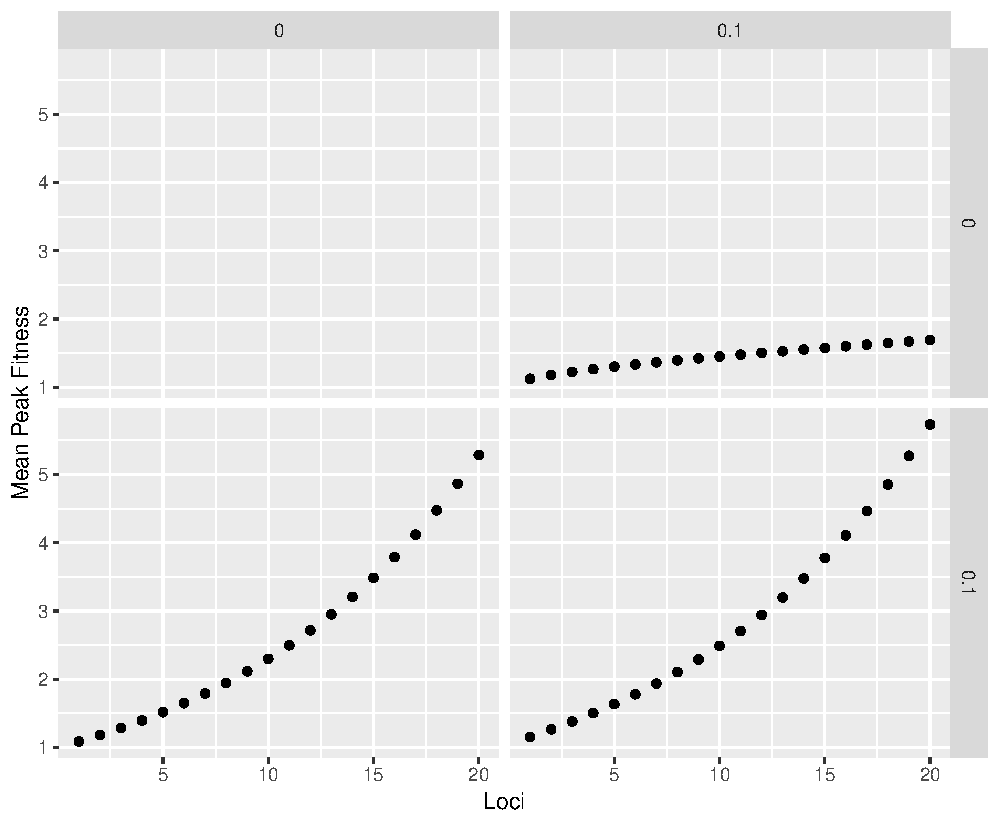
\includegraphics[width = 0.5\textwidth]{figures/mean_peak_scaling.pdf}
	\caption{}
	\label{supp:peak_scaling}
\end{figure}

\begin{figure}[h!]
	\centering
	\subfloat[\label{uf:gt} Fitness trajectories for all simulations, not filtered for genome increasing replicates]{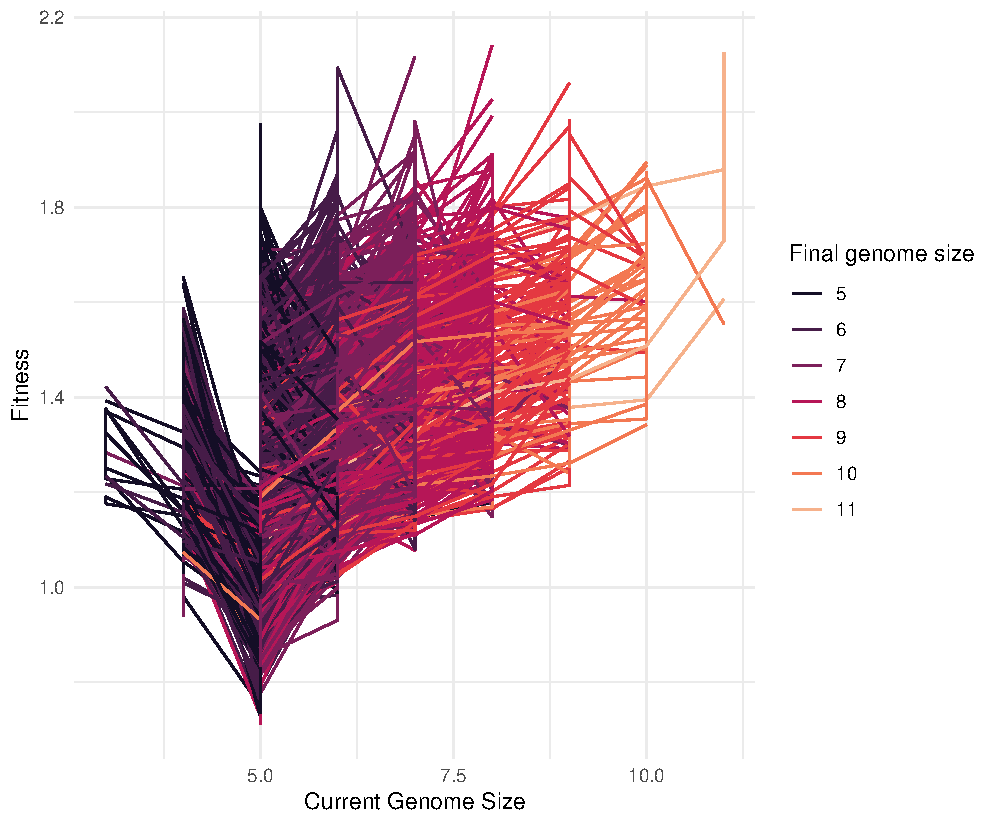
\includegraphics[width = 0.4\textwidth]{figures/genome_trajectories_unfiltered.pdf}}
	\subfloat[\label{uf:bp} Fitness comparisions of endpoint and non-endpoint simulations, unfiltered]{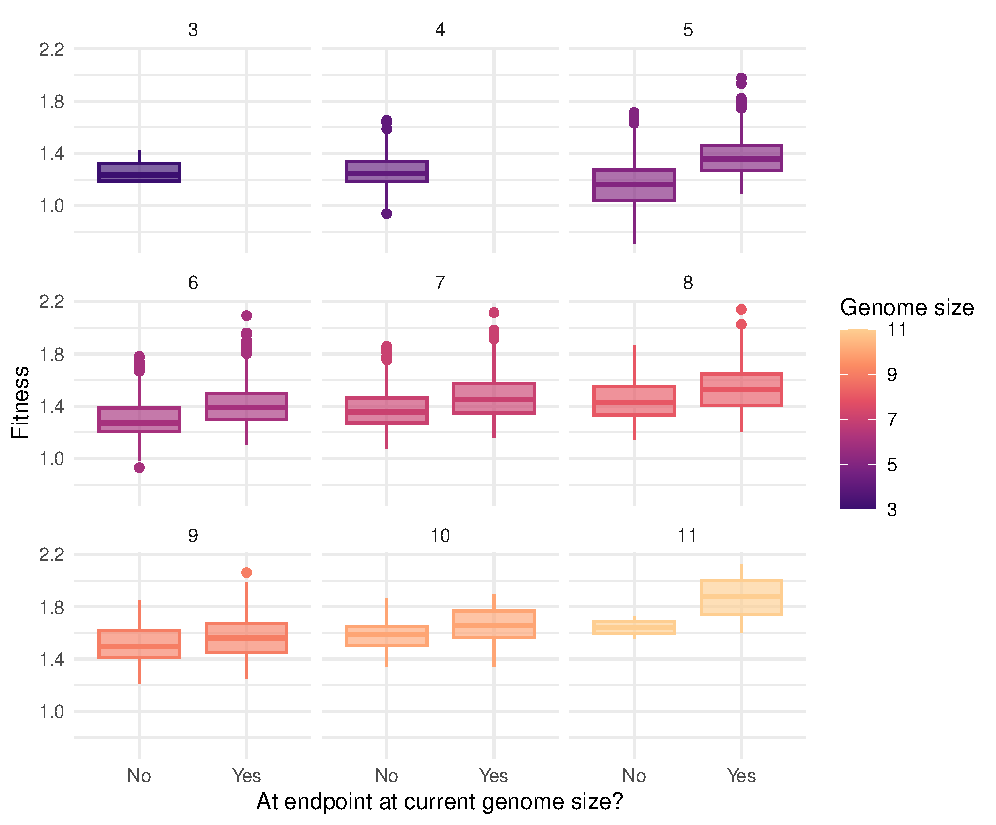
\includegraphics[width = 0.4\textwidth]{figures/endpoint_boxplots_unfiltered.pdf}}
	\caption{}
	\label{uf}
\end{figure}

\end{document}

